\subsection{Competitor}
\subsubsection{G-lock Email Processor} 
\url{http://www.glocksoft.com/email-processor} \\



\begin{figure}[H]
\centering 
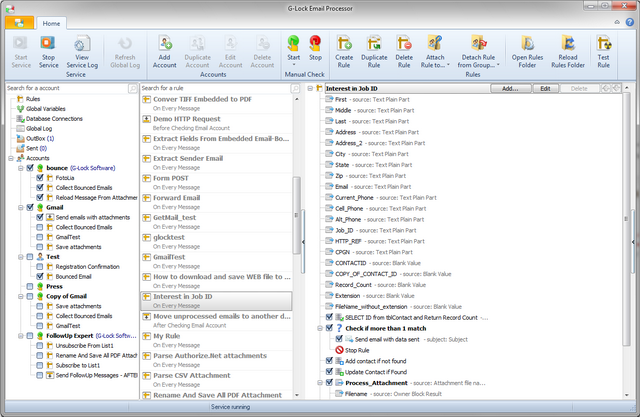
\includegraphics[scale=0.5]{img/gep-main-window-1.png}
\caption{Schermata G-Lock Email Processor}
\end{figure}


Tra i possibili competitor cercando nel web è stato trovato questo software prodotto da una compagnia con sede in Biellorussia che sembra fare quello che viene richiesto.\\
\linebreak Il software è in grado di:
\begin{itemize}
\item Controllare automaticamente il vostro account in modo regolare ed elaborare i messaggi in background 
\item Convertire il contenuto del messaggio in record di database 
\item Salvare i dati estratti dal messaggio in un file 
\item Salvare gli allegati dei messaggi sul disco
\item Creare un report in formato PDF o HTML 
\item Integrare i dati estratti in Microsoft Outlook 
\item Ottimizzare il vostro business ed il servizio al cliente con l'invio di risposte automatiche
\item Convertire automaticamente i dati estratti utilizzando MS Windows script  
\item Estrarre URL da e-mail e processare dati da pagine web e feed RSS 
\end{itemize}

\begin{figure}
\centering 
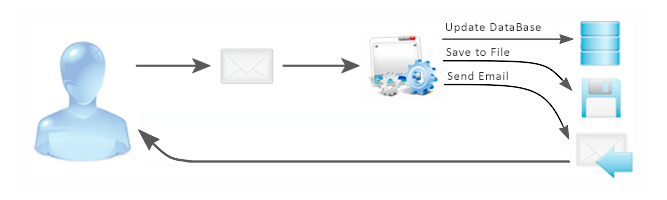
\includegraphics[scale=2.5]{img/emailprocessor.png} 
\caption{Capacità Email Processor}
\end{figure}




Il software si presenta come una possibile soluzione già implementata per quello che stiamo cercando ma risulta avere dei problemi che riguardano le piattaforme per le quali è stato implementato in quanto risulta essere eseguibile solamente su piattaforma Microsoft Windows e questo potrebbe essere un problema in quanto limita il suo possibile uso, inoltre il software risulta essere a pagamento ed avere una spesa di  579,20 USD annui per una licanza di singolo utente.
\newpage

\subsubsection{Email2db}
\url{http://www.email2db.com/email-to-database.aspx}\\
\linebreak


\begin{figure}
\centering 
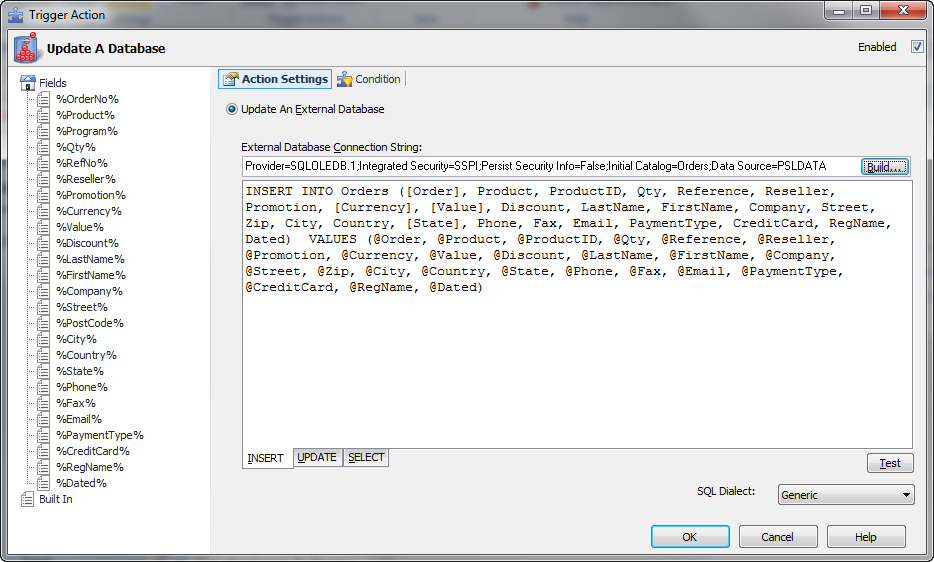
\includegraphics[scale=0.6]{img/email2db.png} 
\caption{Schermata Trigger Email2db}
\end{figure}

Email2DB è un potente strumento per  l'automazione di messaggi che è possibile utilizzare per convertire  email e altri tipi di messaggi in record per database ed inoltre permette di convertire qualsiasi forma di messaggio  anche per Excel o CSV record.\\
\linebreak

Il software è grado di 
\begin{itemize}
\item i leggere messaggi e-mail provenienti da più fonti (Server POP3, Server IMAP, server Exchange, i feed di Twitter, pagine Web, feed RSS e database esterni). 
\item creare un numero qualsiasi di 'Trigger'. Il trigger è un insieme di condizioni che Email2DB verificherà (per esempio, una specifica 'da' l'indirizzo, o parole specifiche nell'oggetto). Se un messaggio supera le condizioni del trigger, Email2DB elaborerà una serie di "azioni" su di essa. Queste azioni comprendono l'aggiornamento di una banca dati, l'invio di eventuali risposte e-mail, report di stampa.
\item analizzare ed estrarre dati da e-mail e aggiornare i tipi di database, tra cui SQL Server, MySQL, Oracle, Pervasive, Access e qualsiasi altro database che supporti ADO o ODBC. 
 \item salvare i dati su foglio di calcolo Excel o file CSV.
\end{itemize}

Email2DB è disponibile in diverse versioni: Small Business, Enterprise, Data Center \& Developer. 

Tutte le edizioni includono le stesse funzionalità per l'analisi e l'estrazione di dati da e-mail per aggiornare più database, permettono di gestire un numero illimitato di account e trigger per l'elaborazione. Inoltre tutte le edizioni non hanno restrizioni sul tipo di messaggi che possono analizzare (Server POP3, IMAP, feed di Twitter) ma per esempio solo le versioni Enterprise e Developer permettono di spostare il messaggio corrente in una cartella diversa da quella in cui è arrivato.
\linebreak

Anche per questo software sorge lo stesso problema del precedente in quando è utilizzabile solo su piattaforme Windows 7/8, Vista, XP, 2003 Server, 2008 Server, 2012 Server. Il software è a pagamento con un costo di 495\euro per la Small Business, 995\euro per la Enterprise, 475\euro per la Developer e 3195\euro per la Data Center Edition ma permette una prova gratuita di 30 giorni dopo essersi registrati.